\documentclass[a4paper,11pt]{article}
\usepackage{titling}
\usepackage[left=2cm, right=2cm, top=2cm]{geometry}
\usepackage{mathtools}
\usepackage{graphicx}
\usepackage{float}
\title{\vspace{-2.0cm}EMP191 Lab 5 - Rocket Launch}
\author{Warren Yuan}
\date{\today}


\begin{document}

\maketitle

\section{Abstract}
\paragraph{\quad In this lab we used the acclerometer to measure accleration of a bottle rocket. The bottle rocket was launched with pressurized air and water from a tube connected to a bike pump. Data was plotted on Matlab. }

\section{Introduction}
\paragraph{\quad The goals of this lab were to understand the acceleration measured and calculate the actual acceleration from the data observed. Using the callibration calculations from last week, and the data observed from this week, we could then plot the graph of acceleration during the flight. }

\section{Measurement Procedure}
\paragraph{\quad Aside from one leaking launch tube, the rocket launch went according to plan. The rocket went very high!}

\section{Plots of Data}
\begin{figure}[H]
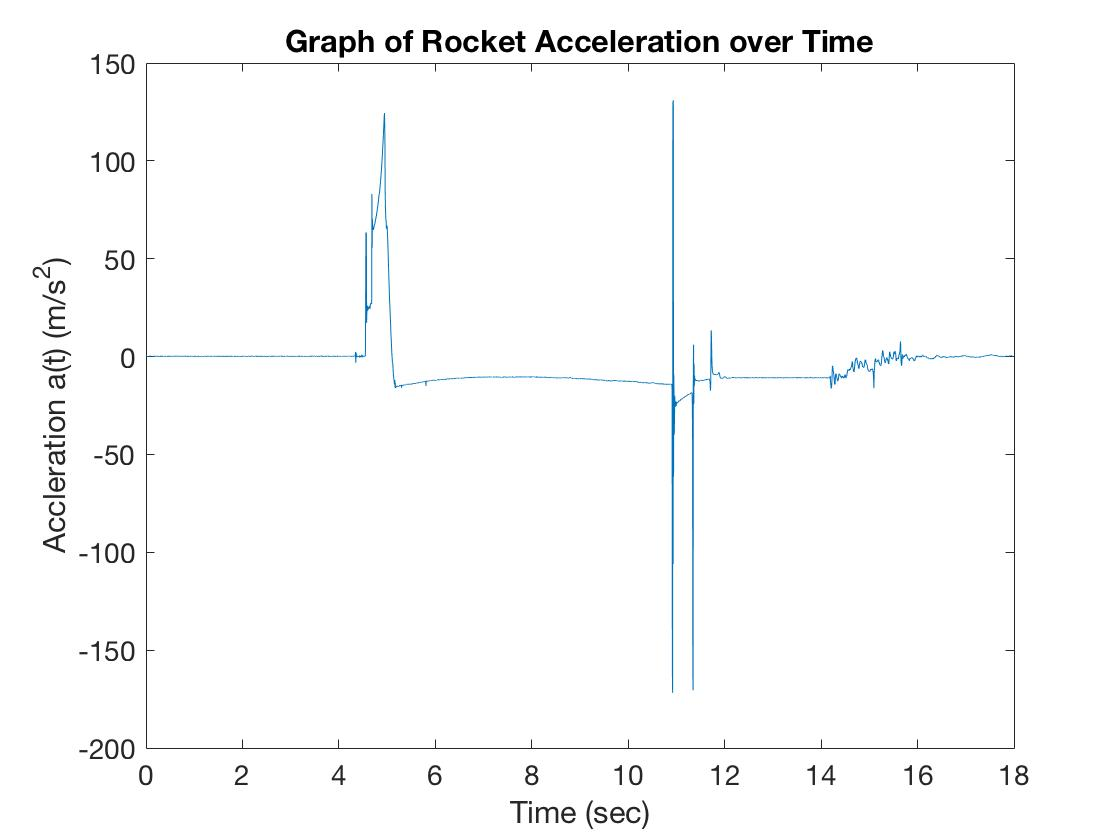
\includegraphics[width=\linewidth/2]{Rocketa(t).jpg}
\end{figure}

\section{Analysis Results}
\paragraph{\quad I recalculated the callibration constant and offset using the upside down and right-side up data right after the launch. I took the average of data from each position to get two equations. I then used the callibration constant and the offset to calculate my actual measured acceleration. I subtracted 9.8 from measured acceleration to get acceleration of the rocket only.}

\begin{equation} 
\textrm{S} = Ca + B
\end{equation}

\paragraph{board right side up}
\begin{equation} 
\textrm{232.8631} = C*(9.8) + B
\end{equation} 

\paragraph{board upside down}
\begin{equation} 
\textrm{-259.1771} = C*(-9.8)+ B
\end{equation} 

\paragraph{Solving the two equations for two unknowns we get: C = 25.10409, B = -13.15704}
\paragraph{From the figure, it is clear to see when the rocket launched as there is a spike in the acceleration which continues until the rocket fuel is spent, a time less than one second. The rocket then coasts for a while, slowly losing velocity (one can see the slight negative acceleration) until it reaches the vertex of the climb, and continues to decelerate. Because acceleration due to gravity was subtracted out, we can see that acceleration is indeed constant (almost zero) on the way down. The large spike at the 11 second mark is the landing, the violent jump is the impact of the rocket hitting the ground, which may have confused the accelerometer, or the rocket bounced on impact. }

\section{Conclusions}
\paragraph{\quad This lab was extremely important for collecting all the data which will eventually be analyzed over the course of the next few weeks. It was integral that the data is not only accurate, but also that the callibration is calculated properly. }
\end{document}
